\begin{frame}{Multivibrador monostável}
\begin{block}{Funcionamento}
O monostável possui um estado estável. Um pulso de disparo gera uma saída temporária e, depois de um tempo definido, o circuito retorna ao repouso.
\end{block}
\begin{center}
\resizebox{0.9\linewidth}{!}{%
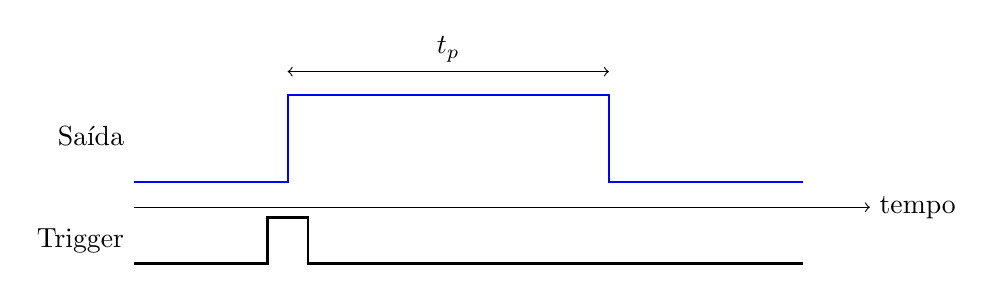
\begin{tikzpicture}[x=.85cm,y=.65cm]
\draw[->] (0,0)--(11,0) node[right]{tempo};
\draw[thick] (0,-1.1)--(2,-1.1)--(2,-.2)--(2.6,-.2)--(2.6,-1.1)--(10,-1.1);
\node[left] at (0,-.65){Trigger};
\draw[thick,blue] (0,.5)--(2.3,.5)--(2.3,2.2)--(7.1,2.2)--(7.1,.5)--(10,.5);
\draw[<->] (2.3,2.65)--node[above]{$t_p$}(7.1,2.65); \node[left] at (0,1.4){Saída};
\end{tikzpicture}%
}
\end{center}
\end{frame}